% 
% process has one thread with two stacks
%  
\chapter{Scheduling}
\label{CH:SCHED}

Any operating system is likely to run with more processes than the
computer has CPUs, so a plan is needed to time-share the
CPUs among the processes. Ideally the sharing would be transparent to user
processes.  A common approach is to provide each process
with the illusion that it has its own virtual CPU by
\indextext{multiplexing}
the processes onto the hardware CPUs.
This chapter explains how xv6 achieves this multiplexing.

Before proceeding with this chapter, please read \lstinline{kernel/proc.h} \fileref{kernel/proc.h},
\lstinline{kernel/swtch.S} \fileref{kernel/swtch.S},
and
{\tt yield()},
{\tt sched()},
and
{\tt scheduler()}
in \lstinline{kernel/proc.c} \fileref{kernel/proc.c}.

%% 
\section{Multiplexing}
%% 

Xv6 multiplexes by switching each CPU from one process to
another in two situations. First, xv6
switches when a process makes a system
call that blocks (has to wait), for example \lstinline{read} or
\lstinline{wait}.
Second, xv6 periodically forces a switch to cope with
processes that compute for long periods without blocking.
The former are called voluntary switches,
the latter involuntary.

Implementing multiplexing poses a few challenges. First, how to switch from one
process to another? 
The basic idea is to save and restore CPU registers,
though the fact that this cannot be expressed in C makes it tricky.
Second, how to force
switches in a way that is transparent to user processes?  Xv6 uses the
standard technique in which a hardware timer's interrupts drive context switches.
Third, all of the CPUs switch among the same set of processes, so a
locking plan is necessary to avoid mistakes such as two CPUs deciding
to run the same process at the same time. Fourth, a process's
memory and other resources must be freed when the process exits,
but it cannot finish all of this itself.
Fifth, each CPU of a multi-core machine must remember which
process it is executing so that system calls affect the correct
process's kernel state.

%% 
\section{Context switch overview}
%% 

The term ``context switch'' refers to the steps involved in a CPU
leaving off execution of one kernel thread (usually for later
resumption), and resuming execution of a different kernel thread; this
switching is the heart of multiplexing. Xv6 does not directly context
switch from one process's kernel thread to another process's kernel
thread; instead, a kernel thread gives up the CPU by context-switching
to that CPU's ``scheduler thread,'' and the scheduler thread picks a
different process's kernel thread to run, and context-switches to that
thread.

\begin{figure}[t]
\center
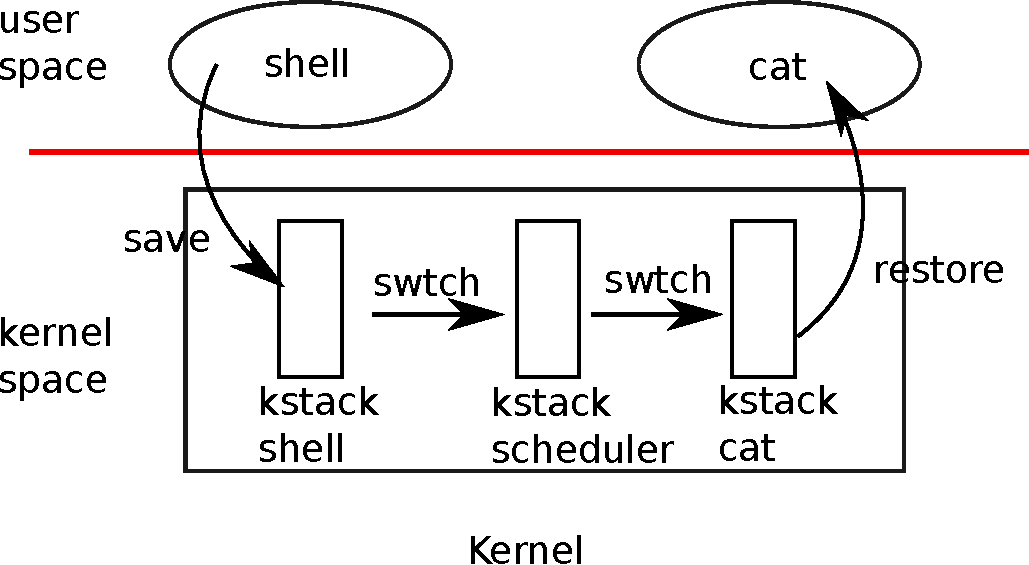
\includegraphics[scale=0.5]{fig/switch.pdf}
\caption{Switching from one user process to another.  In this example, xv6 runs with one CPU (and thus one scheduler thread).}
\label{fig:switch}
\end{figure}

At a broader scope, the steps involved in switching from one user
process to another are illustrated in Figure~\ref{fig:switch}: a trap
(system call or interrupt) from the old process's user space to its
kernel thread, a context switch to the current CPU's scheduler thread,
a context switch to a new process's kernel thread, and a trap return
to the user-level process.


%% 
\section{Code: Context switching}
%% 

The function {\tt swtch()} in {\tt kernel/swtch.S} contains the heart
of thread context switching: it saves the switched-from thread's CPU
registers, and restores the previously-saved registers of the
switched-to thread. The basic reason this is sufficient is that a
thread's state consist of data in memory (e.g. its stack) plus its CPU
registers; thread memory need not saved and restored because different
threads keep their data in different areas of RAM; but the CPU has
only one set of registers so they must be switched (saved and
restored) between threads.

% why must it be in assembler? why not C?
% why swtch(), not switch()?

Each thread's {\tt struct proc} includes a {\tt struct context} that
holds the thread's saved registers when it is not running. A CPU's
scheduler thread's {\tt struct context} is in that CPU's {\tt struct
  cpu}. When thread X wishes to switch to thread Y, thread X
calls {\tt swtch(\&X's context, \&Y's context)}. {\tt swtch()}
saves the current CPU registers in X's context, then loads the content
of Y's context into the CPU registers, then returns.

Here's an abbreviated copy of {\tt swtch}:

\begin{verbatim}
swtch:
        sd ra, 0(a0)
        sd sp, 8(a0)
        sd s0, 16(a0)
        ...
        sd s11, 104(a0)

        ld ra, 0(a1)
        ld sp, 8(a1)
        ld s0, 16(a1)
        ...
        ld s11, 104(a1)
        
        ret
\end{verbatim}

{\tt a0} holds the first function argument, and {\tt a1} the second;
in this case, the two {\tt struct context} pointers.
{\tt 16(a0)} refers to an offset 16 bytes into the memory
pointed to by {\tt a0}; referring
to the definition of {\tt struct context} in {\tt kernel/proc.h}
\lineref{kernel/proc.h:/^struct.context/},
this is the structure field called {\tt s0}.

Where does {\tt swtch}'s {\tt ret} return to? It returns to the
instruction that the {\tt ra} register points to. In the example in
which thread X calls {\tt swtch()} to switch to Y, when {\tt ret}
executes, {\tt ra} has just been loaded from Y's {\tt struct context}.
And the {\tt ra} in Y's {\tt struct context} was originally saved by
Y's call to {\tt swtch} when Y gave up the CPU in the past. So the
{\tt ret} returns to the instruction after the point at which Y called
{\tt swtch()}; that is, X's call to {\tt swtch()} returns as if
returning from Y's original call to {\tt swtch()}. And {\tt sp} will
be Y's stack pointer, since {\tt swtch} loaded {\tt sp} from Y's {\tt
  struct context}; thus on return, Y will execute on its own stack.
{\tt swtch()} need not directly save or restore the program counter;
it's enough to save and restore {\tt ra}.

\lstinline{swtch}
\lineref{kernel/swtch.S:/^swtch:/}
saves callee-saved registers ({\tt ra,sp,s0..s11}) but not caller-saved registers.
The RISC-V calling convention requires that if code needs to
preserve the value in a caller-saved register across a function
call, the compiler must generate instructions
that save the register to the stack before the function call,
and restore from the stack when the
function returns. So \lstinline{swtch} can rely on the function that
called it having already saved the caller-saved registers (either
that, or the calling function didn't need the values in the
registers).

%% 
\section{Code: Scheduling}
%% 

% why a separate thread

The last section looked at the internals of
\indexcode{swtch};
now let's take 
\lstinline{swtch}
as a given and examine 
switching from one process's kernel thread
through the scheduler to another process.
The scheduler exists in the form of a special thread per CPU, each running the
\lstinline{scheduler}
function.
This function is in charge of choosing which process to run next.
Each CPU has its own scheduler thread because more than one CPU may be
looking for something to run at any given time. Process switching
always goes through the scheduler thread, rather than direct from one
process to another, to avoid some situations in which there would be
no stack on which to execute the scheduler (e.g. if the old process
has exited, or there is no other process that currently wants to run).

A process
that wants to give up the CPU must
acquire its own process lock
\indexcode{p->lock},
release any other locks it is holding,
update its own state
(\lstinline{p->state}),
and then call
\indexcode{sched}.
You can see this sequence in
\lstinline{yield}
\lineref{kernel/proc.c:/^yield/},
\texttt{sleep}
and
\texttt{kexit}.
\indexcode{sched}
calls
\indexcode{swtch}
to save the current context in 
\lstinline{p->context}
and switch to the scheduler context in
\indexcode{cpu->context}.
\lstinline{swtch}
returns on the scheduler's stack
as though
\indexcode{scheduler}'s
\lstinline{swtch}
had returned
\lineref{kernel/proc.c:/swtch.*contex.*contex/}.

\lstinline{scheduler}
\lineref{kernel/proc.c:/^scheduler/} 
runs a loop:
find a process to run, {\tt swtch()} to it, eventually it
will {\tt swtch()} back to the scheduler, which continues its loop.
The scheduler
loops over the process table
looking for a runnable process, one that has
\lstinline{p->state} 
\lstinline{==}
\lstinline{RUNNABLE}.
Once it finds a process, it sets the per-CPU current process
variable
\lstinline{c->proc},
marks the process as
\lstinline{RUNNING},
and then calls
\indexcode{swtch}
to start running it
\linerefs{kernel/proc.c:/Switch.to/,/swtch/}.
At some point in the past, the target process must
have called {\tt swtch()}; the scheduler's call to
{\tt swtch()} effectively returns from that
earlier call.
Figure~\ref{fig:inout} illustrates this pattern.

\begin{figure}[t]
\input{fig/switch.tex}
\caption{{\tt swtch()} always has the scheduler thread as either source
or destination, and the relevant {\tt p->lock} is always held.}
\label{fig:inout}
\end{figure}

xv6 holds
\indexcode{p->lock}
across calls to
\lstinline{swtch}:
the caller of
\indexcode{swtch}
acquires the lock,
but it's released in the target after {\tt swtch} returns.
This arrangement is unusual: it's more common for
the thread that acquires a lock to also release it.
Xv6's context switching breaks this convention because
\indexcode{p->state}
and
\lstinline{p->context}
must be updated together atomically.
For example, if
\lstinline{p->lock}
were released before invoking 
\indexcode{swtch},
a different CPU $c$ might decide
to run the process because
its state is \lstinline{RUNNABLE}.
CPU $c$ will invoke \lstinline{swtch}
which will restore from \lstinline{p->context}
while the original CPU
is still saving into
\lstinline{p->context}.
The result would be that the process
would be restored with partially-saved registers on CPU $c$ and
that both CPUs will be using the same stack,
which would cause chaos.
Once \lstinline{yield} has started to modify a running process's state
to make it
\lstinline{RUNNABLE},
\lstinline{p->lock} must remain held until
the process has saved all its registers and
the scheduler is running on its stack.
The earliest correct release point is after
\lstinline{scheduler}
(running on its own stack)
clears
\lstinline{c->proc}.
Similarly, once 
\lstinline{scheduler}
starts to convert a \lstinline{RUNNABLE} process to
\lstinline{RUNNING},
the lock cannot be released until the process's kernel thread
is completely running (after the
\lstinline{swtch},
for example in
\lstinline{yield}).

There is one case when the scheduler's call to
\indexcode{swtch}
does not end up in
\indexcode{sched}.
\lstinline{allocproc} sets the context \lstinline{ra}
register of a new process to
\indexcode{forkret}
\lineref{kernel/proc.c:/^forkret/},
so that its first \lstinline{swtch} ``returns'' 
to the start of that function.
\lstinline{forkret}
exists to release the 
\indexcode{p->lock}
and set up some control registers and trapframe
fields that are required in order to return to user space.
At the end, {\tt forkret} simulates the normal return
path from a system call back to user space.


%% 
\section{Code: mycpu and myproc}
%% 

Xv6 often needs a pointer to the current process's \lstinline{proc}
structure. On a uniprocessor one could have a global variable pointing
to the current \lstinline{proc}. This doesn't work on a multi-core
machine, since each CPU executes a different process. The way to
solve this problem is to exploit the fact that each CPU has its own
set of registers.

While a given CPU is executing in the kernel, xv6 ensures that the CPU's \lstinline{tp}
register always holds the CPU's hartid.
RISC-V numbers its CPUs, giving each
a unique \indextext{hartid}.
\indexcode{mycpu}
\lineref{kernel/proc.c:/^mycpu/}
uses \lstinline{tp} to index an array
of \lstinline{cpu} structures and return the one
for the current CPU.
A
\indexcode{struct cpu}
\lineref{kernel/proc.h:/^struct.cpu/}
holds a pointer to the \lstinline{proc}
structure of
the process currently running
on that CPU (if any),
saved registers for the CPU's scheduler thread,
and the count of nested spinlocks needed to manage
interrupt disabling.

Ensuring that a CPU's \lstinline{tp} holds the CPU's
hartid is a little involved, since user code is free
to modify \lstinline{tp}. \lstinline{start} sets the \lstinline{tp}
register early in the CPU's boot sequence, while still in machine mode
\lineref{kernel/start.c:/w_tp/}.
While preparing to return to user space,
\lstinline{prepare_return} saves \lstinline{tp} in the trampoline
page, in case user code modifies it.
Finally, \lstinline{uservec} restores that saved \lstinline{tp}
when entering the kernel from user space
\lineref{kernel/trampoline.S:/make tp hold/}.
The compiler guarantees never to modify \lstinline{tp}
in kernel code.
It would be more convenient if xv6 could ask the RISC-V
hardware for the current hartid whenever needed,
but RISC-V allows that only in
machine mode, not in supervisor mode.

The return values of
\lstinline{cpuid}
and
\lstinline{mycpu}
are fragile: if the timer were to interrupt and cause
the thread to yield and later resume execution on a different CPU,
a previously returned value would no longer be correct.
To avoid this problem, xv6 requires code to
disable interrupts before calling {\tt cpuid()} or {\tt mycpu()},
and only enable
interrupts when done using the returned value.

The function
\indexcode{myproc}
\lineref{kernel/proc.c:/^myproc/}
returns the
\lstinline{struct proc}
pointer
for the process that is running on the current CPU.
\lstinline{myproc}
disables interrupts, invokes
\lstinline{mycpu},
fetches the current process pointer
(\lstinline{c->proc})
out of the
\lstinline{struct cpu},
and then enables interrupts.
The return value of
\lstinline{myproc}
is safe to use even if interrupts are enabled:
if a timer interrupt moves the calling process to a
different CPU, its
\lstinline{struct proc}
pointer will stay the same.


%% 
\section{Real world}
%% 

The xv6 scheduler implements a simple scheduling policy that runs each process
in turn.  This policy is called
\indextext{round robin}.
Real operating systems implement more sophisticated policies that, for example,
allow processes to have priorities.  The idea is that a runnable high-priority process
will be preferred by the scheduler over a runnable low-priority process.   These
policies can become complex because there are often competing goals: for
example, the operating system might also want to guarantee fairness and
high throughput.

%% 
\section{Exercises}
%% 

\begin{enumerate}

\item Modify xv6 to use only one context switch when switching from
  one process's kernel thread to another, rather than switching
  through the scheduler thread. The yielding thread will need to select
  the next thread itself and call \texttt{swtch}. The challenges will
  be to prevent multiple CPUs from executing the same thread accidentally;
  to get the locking right; and to avoid deadlocks.

\end{enumerate}
